\documentclass[10pt, hyperref={pdfpagelabels=false}]{beamer}

\usepackage{tikz, verbatim, enumitem}

\usetikzlibrary{decorations}
\usetikzlibrary{backgrounds}
\usetikzlibrary{patterns}
\usetikzlibrary{snakes}
\usetikzlibrary{shapes}
\usetikzlibrary{positioning, shapes.geometric, arrows.meta}
\usetikzlibrary{arrows,automata}

\setlength{\parindent}{0pt}
\setlength{\parskip}{1.3ex}

\title{Authentication: Integrity Checking}
\author{Michael Brockway}
\date{\today}

\setlist[enumerate]{itemsep=0mm}
\setitemize{label=\usebeamerfont*{itemize item}
  \usebeamercolor[fg]{itemize item}
  \usebeamertemplate{itemize item}}

\begin{document}

\begin{frame}
\titlepage
\end{frame}

\begin{frame}
\frametitle{Overview}
We have met two ways in which we need to be assured or the \emph{authenticity} of a message sent through a network:
\begin{itemize}
\item The message really is from the party who purportedly sent it; 
\item The message data is as sent; it has not been tampered with en route. 
\end{itemize}

These are two different security assurances and we seen one is provided for by a digital signature mechanism (backed up by digital certificates) while the other is provided a \emph{message digest} created by a \emph{hash function}.

The acronym MAC, 'Message authentication code' is confusingly used to refer to either of these. These slides focus of the second and takes a closer look at message digests and hash functions.
\end{frame}

\begin{frame}
\frametitle{Hash Functions}
\begin{center}
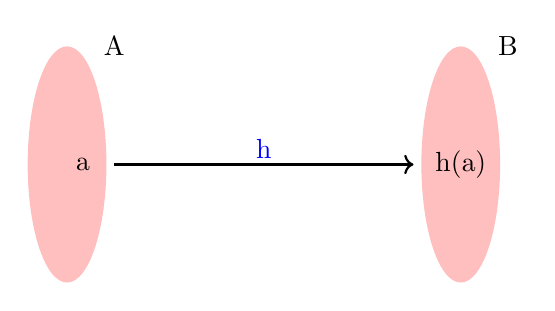
\begin{tikzpicture} [ball/.style={ellipse, minimum width=1, minimum height=4, draw, >=LaTeX}]
\fill[color=pink] (0,0) circle [x radius = 5mm, y radius = 15mm];
\fill[color=pink] (5,0) circle [x radius = 5mm, y radius = 15mm];
\draw (0.6,1.5) node {A}; \draw (5.6,1.5) node {B};
\draw (0.2,0) node {a}; \draw (5.0,0) node {h(a)};
\draw[->, thick] (0.6,0) -- (4.4,0); 
\draw (2.5,0.2) node[color=blue] {h};
\end{tikzpicture}
\end{center}
In general, a \emph{function} $h$ maps a set $A$ of objects to a set $B$ of (other) objects, the idea being that for any $a \in A$ there is a (\emph{unique}) $h(a) \in B$. We write $A \stackrel{h}{\rightarrow} B$.

An example: any java Object \texttt{ob} has a method:\\
\texttt{\color{blue}public int ob.hashCode()}.\\
We can think of $h$ mapping \texttt{ob} to \texttt{ob.hashCode()}. In this case $B$ is the set of \texttt{int} values - there are $2^{32}$ of them.
\end{frame}

\begin{frame}
\frametitle{Hash Functions}
Java hash functions are supposed to be contrived so that whenever \texttt{\color{blue}(ob1.equals(ob2))} then \texttt{\color{blue}(ob1.hashCode() == ob1.hashCode())}. To be useful, we would also like\\
\texttt{\color{blue}(!ob1.equals(ob2))} $\Rightarrow$ \texttt{\color{blue}(ob1.hashCode() != ob1.hashCode())}.

This is not guaranteed but a \emph{\color{blue}hash collision}, where \texttt{\color{blue}(!ob1.equals(ob2))} but \texttt{\color{blue}(ob1.hashCode() == ob1.hashCode())} has very low probability when the hash function is well designed.

Java programmers overriding Object.hashCode() are supposed to pay attention to this.
\end{frame}

\begin{frame}
\frametitle{Hash Functions}
You have met java \texttt{HashSet}s and \texttt{HashMap}s which store objects in \emph{hash tables}.
\begin{itemize}
\item A suitably contrived hash function on objects returns a number which indexes into an array.
\item The object reference is stored here;
\item A collision is resolved by putting the objects in a linked list at the location.
\item If the probability of the collision is low than these lists are short.
\end{itemize}
\end{frame}

\begin{frame}
\frametitle{Cryptographic hash functions}
\begin{center}
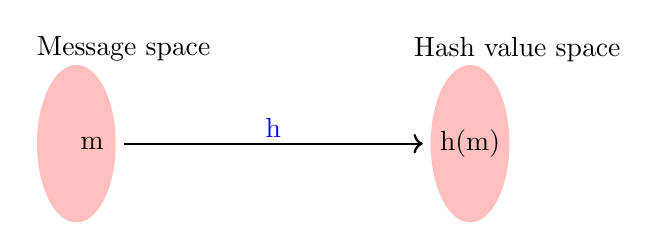
\begin{tikzpicture} [ball/.style={ellipse, minimum width=1, minimum height=4, draw, >=LaTeX}]
\fill[color=pink] (0,0) circle [x radius = 5mm, y radius = 10mm];
\fill[color=pink] (5,0) circle [x radius = 5mm, y radius = 10mm];
\draw (0.6,1.2) node {Message space}; \draw (5.6,1.2) node {Hash value space};
\draw (0.2,0) node {m}; \draw (5.0,0) node {h(m)};
\draw[->, thick] (0.6,0) -- (4.4,0); 
\draw (2.5,0.2) node[color=blue] {h};
\end{tikzpicture}
\end{center}

For every message $m$, hash value $h(m)$ is efficiently computable: it is a sequence bits which can be thought of as an integer: $h(m) < 2^s$ where is $s$ is the size of the hash in bits.
\begin{itemize}
\item Not only are hash collisions improbable ($2^s$ is `large'), but a 1-bit change in the message almost always produces a large change in h(m);
\item $h$ is \emph{\color{blue}pre-image resistent}: it is infeasible (for an attakcer) to contrive a message $m$ for which $h(m) =$ a desired value - such as the hash of another message;
\item It is \emph{\color{blue}strongly collision resistant}: it is infeasible to contrive a pair of messages $m, m'$ such that $h(m) == h(m')$.
\end{itemize}
\end{frame}

\begin{frame}
\frametitle{Cryptographic hash functions - use}
\begin{itemize}
\item The sender of a message computes the hash of the message and appends it before encrypting.
\item The recever, after decrypting, computes a hash,
\item and compares it with the one that was sent.
\item Any mismtch $=>$ tampering!
\end{itemize}
\end{frame}

\begin{frame}
\frametitle{Cryptographic hash functions}
\small
The \emph{\color{blue}birthday attack} is an exploit protected against by strongly collision-resistant hashing. The attacker has two versions of, say, a contract, one less favourable than the other, with the same hash value, and can switch them without detection if the hash were \emph{not} strongly collision-resistant.

You have probably heard that in a random sample of $n$ people, the probability two have birthdays on the same day grows with $n$ and passes 0.5-0.5 when $n>23$...

\begin{figure}
\includegraphics[width=0.8\textwidth]{birthdayCollision.eps}
\end{figure}
\end{frame}

\begin{frame}
\frametitle{Cryptographic hash function examples - MD5}
MD5 (R Rivest, 1991-2)
\begin{itemize}
\item 128-bit hashes: $2^{128} \approx 10^{38}$, 100 million million million million million million values; 
\item by 2004, not enough! Wang, Feng, Lai and Yu contrived a collision in 1 CPU-hour on an IBM p690
\item Updates were issued until 2010
\item Now considered insecure, also found to be still used as recently as 2015.
\item The Wikipedia article has a neat summary of the algorithm, its security issues and vularabilities. 
\end{itemize}
\end{frame}

\begin{frame}
\frametitle{SHA-1: Secure hash algorithm 1}
\begin{itemize}
\item 160-bit hashes: $2^{160} \approx 1.4 \times 10^{48}$, a million million million million million million million million values; 
\item From 2005, collision attacks began to be contrived: Rijmen and Oswald in $2^{80}$ operations, Wang, Yin and Yu in $2^{69}$ operations.
\item These early attacks were actually prohibitively expensive; but in October 2015 M Stevens and others \emph{demonstrated} a partial attack using a grid of NVIDIA GPUs costing around US\$2000 - 
\item ... and in Feb 2017 the \emph{SHAttered} attack (CWI and Google) ...
\end{itemize}
\texttt{\small\color{blue}https://www.theregister.co.uk/2017/02/23/google\_first\_sha1\_collision/}
\begin{itemize}
\item generated two different PDF files with the same SHA-1 hash in roughly $2^{63.1}$ SHA-1 evaluations. 
\item 100,000 times faster than brute force birthday attack
\item required equivalent of 6,500 years of single-CPU computations or 110 years of single-GPU computations
\end{itemize}

The Wikipedia article has a neat summary of the algorithm, its security issues and vularabilities. 
\end{frame}

\begin{frame}
\frametitle{SHA-2 family}
\begin{itemize}
\item SHA-224, 256, 384, 512, 512/224, 512/256 (USA NSA)
\item SHA-256, for instance outputs a 256-bit number: $2^{256} \approx 10^{77}$ values; currently recommended for TLS although already attacks are being show to be possible.
\item A SHA-256 hash is handled as an array of 8 32-bit words (unsigned integers).
\item SHA-512 which works with 64-bit words is coming to be recommended for 64 bit machines.
\end{itemize}

SHA-256 is considered in more detail below and is in a sense typical of this family of hash functions. SHA512 follows similar logic but a `state' consists of 8 x 64- rather than 32-bit words.
\end{frame}

\begin{frame}
\frametitle{SHA-256}
The 256-bit hash is handled as an array of 8 x 32-bit integers. These are called \emph{words} in the literature:
\begin{itemize}
\item in C they would have type \texttt{unsigned int} or \texttt{uint32\_t}
\item in Java, just \texttt{int}
\end{itemize}

The data is organized as 512-bit (64 byte, 16 word) \emph{\color{blue}blocks}. A high-level view of the process is:
\begin{itemize}
\item The hash is initialized;
\item There is a \emph{round} for each block:
  \begin{itemize}
  \item an update to the hash is computed (as 8 words) and
  \item added, word-wise, to the hash
  \end{itemize}
\item Done, once all blocks have been processed. The hash is returned.
\end{itemize}
\end{frame}

\begin{frame}
\frametitle{SHA-256 helpers}
The SHA-256 algorithm employs some constants -
\begin{itemize}
\item \texttt{\color{brown}word[8] hashInit}, array of 8 x 32-bit constants to initialise the hash;
\item \texttt{\color{brown}word[64] roundConst}, array of 64x32-bit constants used in each round.
\end{itemize}

Some bitwise logic functions -
\begin{itemize}
\item \texttt{\color{brown}word rotr(word wd, int k) \{\\~~return (wd >> k) | (wd << (32-k)); \}} - rotate wd k bits to right
\item \texttt{\color{brown}word ch(word x, word y, word x) \{\\~~return (x \& y) \^{} ($\sim$x \& z); \}} - think `choice'
\item \texttt{\color{brown}word maj(word x, word y, word x) \{\\~~return (x \& y) \^{} (x \& z) \^{} (y \& z); \}} - think `majority' 
\end{itemize}
\end{frame}

\begin{frame}
\frametitle{SHA-256 helpers}
Some `magic' functions used in block (round) processing -
\begin{itemize}
\item \texttt{\color{brown}word $\Sigma_0$(word x) \{\\~~return rotr(x,2) \^{} rotr(x,13) \^{} rotr(x,22); \}} 
\item \texttt{\color{brown}word $\Sigma_1$(word x) \{\\~~return rotr(x,6) \^{} rotr(x,11) \^{} rotr(x,25); \}} 
\item \texttt{\color{brown}word $\sigma_0$(word x) \{\\~~return rotr(x,7) \^{} rotr(x,18) \^{} (x >> 3); \}} 
\item \texttt{\color{brown}word $\sigma_1$(word x) \{\\~~return rotr(x,17) \^{} rotr(x,19) \^{} (x >> 10); \}} 
\end{itemize}
\end{frame}

\begin{frame}
\frametitle{SHA-256 block setup and hash initialisation}
The input data has to be a whole number of 16-word blocks. This contrived by add padding in the following form -
\begin{itemize}
\item a 1 bit
\item some 0 bits
\item a 64-bit unsigned integer: the number of bits of data input.
\end{itemize}

The number of 0-bits in the padding is just what is needed to get the overall bit size a multiple of 512 (ie, 16 words).

The data does not have to be all input at this stage - it can be input on the fly during block processing rounds but the data length needs to be known in advance to set up the padding. 

The hash (array of 8 words) it initialised to a copy of \texttt{\color{brown}hashInit}. 
\end{frame}

\begin{frame}
\frametitle{SHA-256 block processing rounds}
The data is a whole number of 16-word blocks. For each block,
\begin{itemize}
\item a 64-word array \texttt{\color{brown}w} is created from the data:
  \begin{itemize}
  \item \texttt{\color{brown}w[0..15]} is copied from the 16 words of the block;
  \item for i = 16 to 63 set \texttt{\color{brown}w[i] =\\~~$\sigma_1$(w[i-2]) + w[i-7] + $\sigma_0$(w[i-15]) + w[i-16]}
  \end{itemize}
\item the hash value from the previous round (in the first round, the initial value) is copied to 8 words excitingly denoted $a, b, c, d, e, f, g, h$;
\item For i = 0 to 63,\\~~these variables are updated using \texttt{\color{brown}w[i]} and \texttt{\color{brown}roundConst[i]} as indicated ($w_i, k_i$) in the diagram below;
\item the 64-times updated $a, ..., h$ are added modulo $2^{32}$ to the hash words:\\
\texttt{\color{brown}hash[0] += a; hash[1] += b; ...; hash[7] += h;}
\end{itemize}
NB `+', addition of words, is modulo $2^{32}$. Note also we have here a 64x iteration within each block - there are potentially many iterations.
\end{frame}

\begin{frame}
\frametitle{SHA-256 block processing: $i^{th}$ update of $a...h$}
\begin{center}
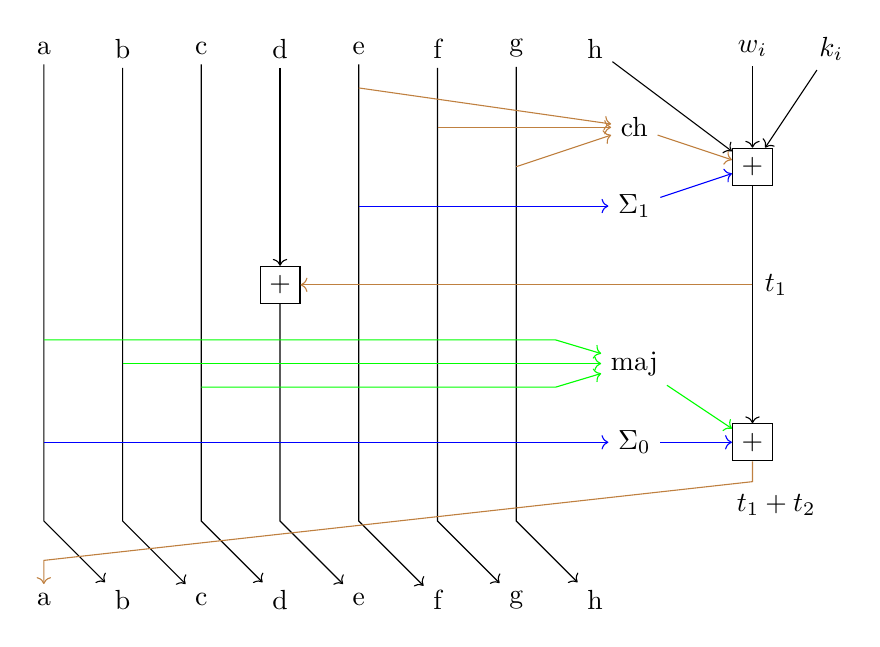
\begin{tikzpicture}
  \draw (0,8) node (a0) {a}; \draw (1,8) node (b0) {b};
  \draw (2,8) node (c0) {c}; \draw (3,8) node (d0) {d};
  \draw (4,8) node (e0) {e}; \draw (5,8) node (f0) {f};
  \draw (6,8) node (g0) {g}; \draw (7,8) node (h0) {h};

  \draw (3,5) node[draw] (pd) {+};

  \draw (0,1) node (a2) {a}; \draw (1,1) node (b2) {b};
  \draw (2,1) node (c2) {c}; \draw (3,1) node (d2) {d};
  \draw (4,1) node (e2) {e}; \draw (5,1) node (f2) {f};
  \draw (6,1) node (g2) {g}; \draw (7,1) node (h2) {h};

  \draw[black, ->] (a0) -- (0,2) -- (b2);
  \draw[black, ->] (b0) -- (1,2) -- (c2);
  \draw[black, ->] (c0) -- (2,2) -- (d2);
  \draw[black, ->] (d0) -- (pd);
  \draw[black, ->] (pd) -- (3,2) -- (e2);
  \draw[black, ->] (e0) -- (4,2) -- (f2);
  \draw[black, ->] (f0) -- (5,2) -- (g2);
  \draw[black, ->] (g0) -- (6,2) -- (h2);

  \draw (9,8) node (w) {$w_i$}; \draw (10,8) node (k) {$k_i$};

  \draw (9,6.5) node[draw] (p0) {+};
  \draw[black, ->] (w) -- (p0); \draw[black, ->] (k) -- (p0); 
  \draw[black, ->] (h0) -- (p0); 

  \draw (7.5,7) node (ch) {ch};
  \draw[brown, ->] (4,7.5) -- (ch);
  \draw[brown, ->] (5,7.0) -- (ch);
  \draw[brown, ->] (6,6.5) -- (ch); \draw[brown, ->] (ch) -- (p0);

  \draw (7.5,6) node (s1) {$\Sigma_1$};
  \draw[blue, ->] (4,6) -- (s1); \draw[blue, ->] (s1) -- (p0);

  \draw (9,3) node[draw] (p1) {+}; \draw[black, ->] (p0) -- (p1);
  \draw[brown, ->] (9,5) -- (pd);
  \draw (9.3,5) node {$t_1$};

  \draw (7.5,4) node (mj) {maj}; \draw[green, ->] (1,4) -- (mj);
  \draw[green, ->] (0,4.3) -- (6.5,4.3) -- (mj);
  \draw[green, ->] (2,3.7) -- (6.5,3.7) -- (mj);
  \draw[green, ->] (mj) -- (p1);

  \draw (7.5,3) node (s0) {$\Sigma_0$};
  \draw[blue, ->] (0,3) -- (s0); \draw[blue, ->] (s0) -- (p1);

  \draw[brown, ->] (p1) -- (9,2.5) -- (0,1.5) -- (a2);
  \draw (9.3,2.2) node {$t_1+t_2$};

\end{tikzpicture}
\end{center}

\end{frame}

\begin{frame}
\frametitle{Further reading}
\begin{itemize}
\item \texttt{\small\color{blue}https://en.wikipedia.org/wiki/MD5}
\item \texttt{\small\color{blue}https://en.wikipedia.org/wiki/SHA-1}
\item \texttt{\footnotesize https://www.theregister.co.uk/2017/02/23/google\_first\_sha1\_collision/}
\item \texttt{\small\color{blue}https://en.wikipedia.org/wiki/SHA-2}
\item \texttt{\footnotesize http://www.iwar.org.uk/comsec/resources/cipher/sha256-384-512.pdf}
\item Here is a zip containing java implementations of SHA-1 (mainly of historical interest now!) and SHA-256:\\
 \texttt{\small\color{blue}http://computing.northumbria.ac.uk/staff/cgmb3/teaching/\\cryptography/SecureHashAlgs.zip}\\
\texttt{Sha256.java} lines 255-282 cover processing a block; 266-277 correspond to the diagram.
\end{itemize}
\end{frame}

\end{document}

